\chapter{Synthesis}
The overarching goal of this thesis is to develop a combined earthquake catalog for the Ngatamariki and Rotokawa geothermal fields in New Zealand, and to use it as a tool for reservoir characterization. This catalog of industrially-induced seismicity is a manifestation of temperature and pressure change within the earth and therefore represents an opportunity to study these properties within a geothermal resource, where no direct measurements can be made. The work contained herein comprises detailed analyses of seismicity beyond the day-to-day monitoring conducted by the geothermal operators, specifically focusing on areas and time periods of intense fluid injection operations. It is our intent that the results presented in this work be of practical use to Mercury NZ, Ltd, from the standpoint of reservoir management and planning at these fields.

\section{Summary}
The earthquake catalog presented in this thesis was constructed from a single network of continuously-recording seismographs. However, as this project concerns two separate geothermal fields with distinct development histories, our analyses have been partitioned into two parts, one for Ngatamariki (Chapter 3) and one for Rotokawa (Chapter 4) with a final, combined portion discussing focal mechanisms and stress state at both fields (Chapter 5). Chapter 3 presents the Ngatamariki earthquake catalog and analyzes its characteristics in relation to injection well drilling and stimluation prior to plant startup. Chapter 4 presents the Rotokawa earthquake catalog and discusses spatio-temporal trends in rate, location and frequency-magnitude distribution revealed therein. Chapter 5 addresses the focal mechanisms and stress state at both fields.

\begin{flushleft}
The specific findings of each chapter are summarized below:
\end{flushleft}

\begin{flushleft}
Chapter 3:
\end{flushleft}
\begin{itemize}
    \item We applied a matched-filter detection algorithm to continuous seismic data at the Ngatamariki and Rotokawa geothermal fields to increase the total number of events in our catalog;
    \item Seismicity at Ngatamariki from 2012--2015 occurs in two clusters, spatially coincident with the northern and southern injection zones. Little seismicity occurs in the production field;
    \item Drilling, testing and \gls{stimulation} treatments at wells NM08, NM09 and NM10 produce dramatically different responses in seismicity;
    \item The rate of seismicity and \acrfull{II} increase are poorly correlated during injection well \gls{stimulation} at NM08 and NM09;
    \item Stress inversions from earthquake focal mechanisms reveal distinct stress states in the northern and southern injection zone.
\end{itemize}\par

\begin{flushleft}
Chapter 4:
\end{flushleft}
\begin{itemize}
    \item Seismicity at Rotokawa from 2012--2015 is confined to the injection field, bounded to the northwest by the \acrfull{CFF}. This pattern in consistent with previous studies of seismicity in the field \citep{Sherburn_2015,Sewell_2015WGC};
    \item Our catalog reveals, for the first time, two distinct, sub-linear features within the seismically-active portion of the field. From west to east, we infer these features to be the \acrshort{CFF} and \acrfull{IFF};
    \item Mapping of earthquake frequency-magnitude distribution (i.e. $b$-value) reveals a complex pattern in the Rotokawa injection field. Areas of elevated pore pressure and high degree of fracturing may correspond to areas of high $b$-value.  
\end{itemize}\par

\begin{flushleft}
Chapter 5:
\end{flushleft}
\begin{itemize}
    \item We calculated 982 focal mechanism solutions for Ngatamariki (205) and Rotokawa (777) from 2012--2015, exhibiting predominantly normal, with a lesser number of strike-slip events;
    \item Stress inversions from kmeans clusters at Ngatamariki reveal a pure normal-faulting regime in southern Ngatamariki and an unconventional regime in the north in which no principle stress is vertical;
    \item Discrepancies between stress results within the northern injection zone may be related to thermal cooling and contraction of the reservoir;
    \item Stress inversion results at Rotokawa indicate a uniformly normal stress regime across the seismically-active portion of the reservoir;
    \item Temporal variations in the stress ratio, $\nu$, near the main injection wells may reflect changes in the shape of the cooled zone of the reservoir.
\end{itemize}\par

Below, we discuss the implications of these findings, focusing on each field individually.

\subsection{Ngatamariki}
The portion of this thesis pertaining to Ngatamariki represents the first detailed study of seismicity at the field. Using an automatically-detected and located earthquake catalog provided by GNS Science as templates, we applied a matched-filter detection approach in order to increase the total number of events in our catalog. The Ngatamariki catalog analyzed in this thesis contains over 2500 precisely-located events spanning nearly four years during initial development and plant startup.

At each step in our analysis, the distinction between the northern and southern injection zones at Ngatamariki is emphasized. Although \glspl{flow_rate} and \glspl{WHP_g} in each zone are similar, the seismic response of the reservoir is not. Seismicity in the north has both a higher $b$-value (1.84 vs. 1.20) and a more oblate spatial footprint. Additionally, stress inversion results from focal mechanisms in the north reveal an unconventional stress state with no vertical axes, whereas stress results in the south show the expected normal-faulting regime with NE-SW S$_{Hmax}$. The two zones of the reservoir are known to be geologically distinct \citep{Bignall_2009,Chambefort_2014} and this may help explain the differences in seismicity. The southern injection wells intersect a structure inferred to be related to the Aratiatia Fault Zone (Figure \ref{seis_overview}), a large, kilometers-long structure that can accommodate large ruptures. The north is highly-fractured and dominated by a tonalite intrusive body (below $\sim$2000 m bsl) of unknown spatial extent. We infer the higher $b$-value in the north to be a result of pervasive fracturing associated with the emplacement of the intrusive, resulting in a higher concentration of fractures of shorter length and thereby limiting the likelihood of large-magnitude seismicity.

\begin{figure}[h!]
\begin{center}
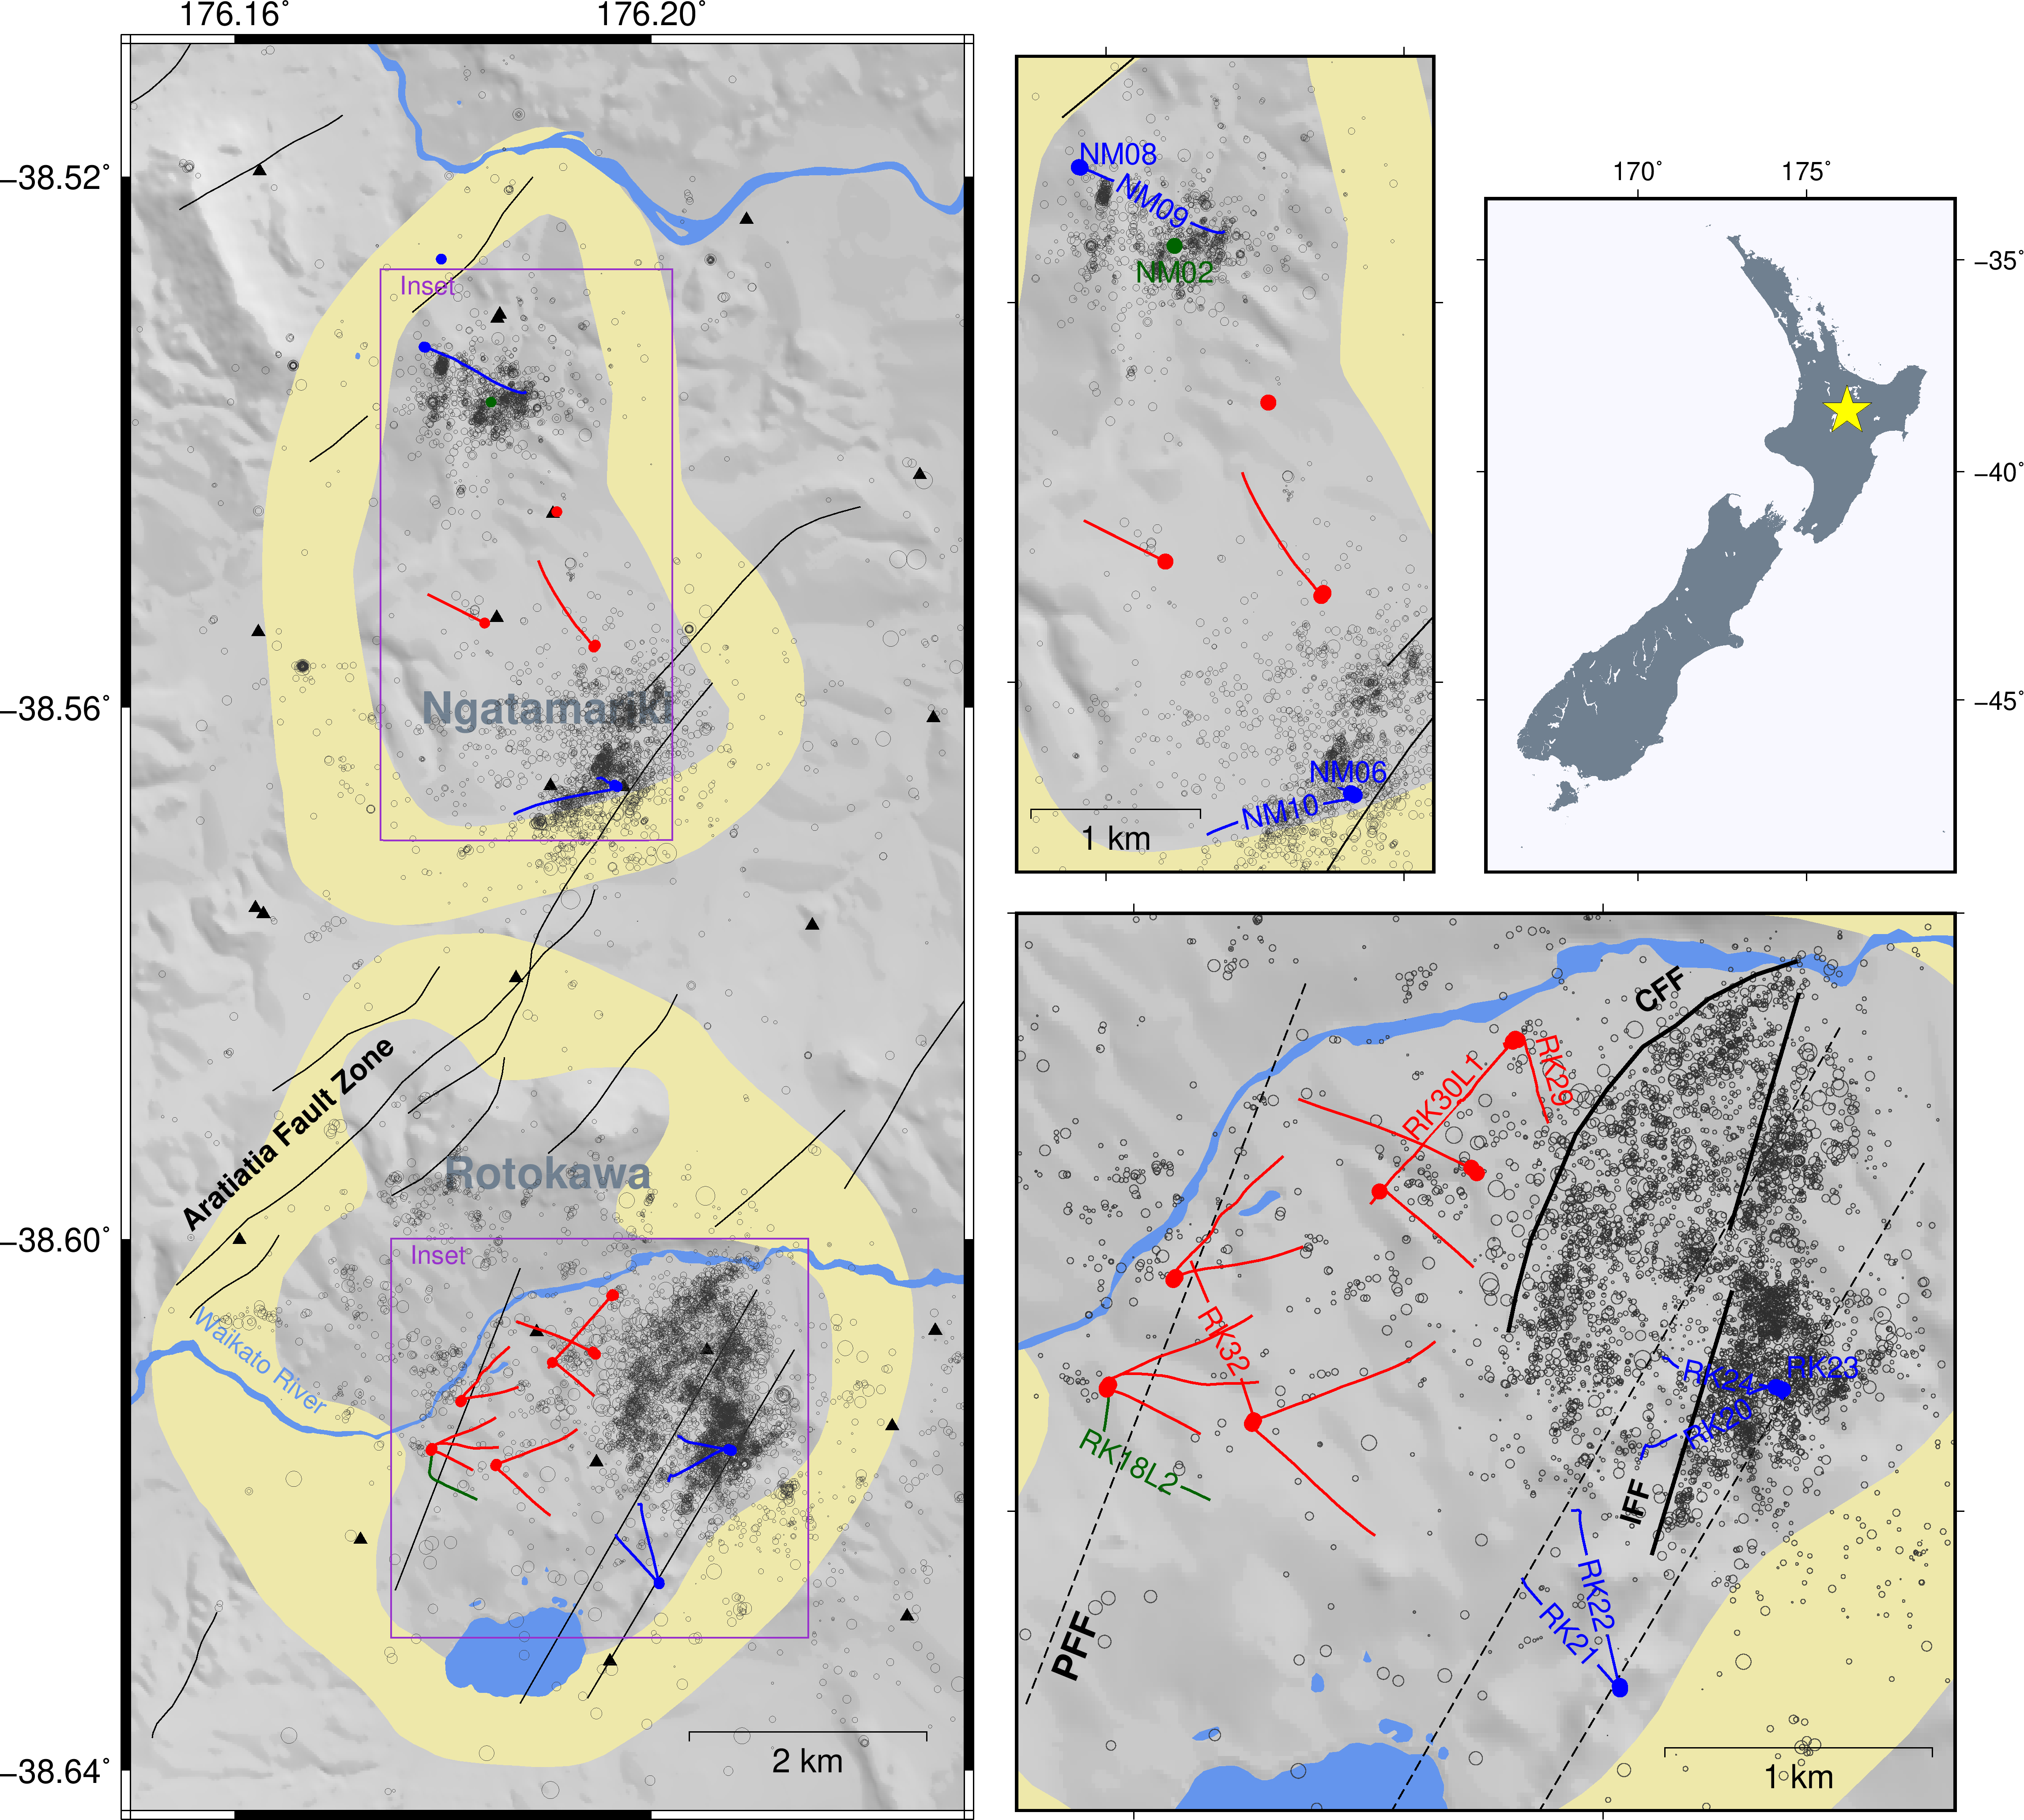
\includegraphics[width=1.00\columnwidth]{Chapter_6_Synthesis/figures/overview_seis/merc_RotNga_overview_seis_chap6}
\caption[The combined Ngatamariki-Rotokawa seismic catalog]{{
Overview of the combined, Ngatamariki-Rotokawa seismic catalog presented in this thesis. Yellow polygons define the outlines of the resources and black lines represent active faults \citep{AFDB}. Black circles are seismic events with the radius of each symbol proportional to the magnitude. Blue, red and green lines are injection, production and monitoring wells, respectively. In the Rotokawa inset (lower right panel) dotted lines represent the previously-modeled orientations of the \acrshort{PFF}, \acrshort{CFF} and \acrshort{IFF}. The bold black lines indicate the modified orientations for the \acrshort{CFF} and \acrshort{IFF} inferred in this thesis from the location of seismicity.
{\label{seis_overview}}%
}}
\end{center}
\end{figure}\selectlanguage{english}

We infer the stress state variation between the northern and southern injection zones to also be a result of the emplacement of the intrusive body. However, within the northern zone, stress field variations may also be a result of injection operations. We have detailed a scenario in Section 5.4.1, through which the shape of the cooled zone of the reservoir would preferentially decrease $\sigma_{1}$, thereby significantly altering the reservoir stress state, as has been observed and modeled elsewhere \citep{Mart_nez_Garz_n_2013,Jeanne_2015tensor}.

We have also conducted a detailed spatio-teporal analysis of seismicity during pre-startup drilling and \gls{stimulation} operations at Ngatamariki. These results suggest that \acrfull{II}, a proxy for \gls{permeability} increase, during injection operations is poorly correlated with both the location and rate of associated seismicity. This result agrees with recent work by \citet{Riffault_2018}, showing that \acrshort{II} is not necessarily a result of seismic slip on preexisting fractures, but instead may be dominated by near-well, aseismic fracture slip\slash{opening} near the wellbore. We infer this to be the case during the \gls{stimulation} of NM08 in northern Ngatamariki, where \acrshort{II} increases throughout the treatment but seismicity is induced only after a week of injection. In addition, injection well NM09, which is seismically active after plant startup, induced no observed seismic events during pre-startup \gls{stimulation} and injection testing. However, \acrshort{II} increased throughout this treatment, leading to the simple conclusion that the observed \gls{permeability} increase was not due to seismic slip.

\subsection{Rotokawa}
Previous studies of Rotokawa seismicity by \citet{Sherburn_2015} and \citet{Sewell_2015WGC} identified an area of active seismicity (as of 2012) in the northeast part of the field, between the northern injection wells and northern production wells, extending NE towards the field boundary. The catalog presented here, from 2012--2015, shows a broadly similar seismically-active area. Where the catalog of \citet{Sherburn_2015} and \citet{Sewell_2015WGC} showed only a single microseismic cloud, our catalog is able to distinguish between different structures. From our high-precision locations of nearly 6500 events, we infer a modified location for the \acrfull{CFF}, located northwest of its previously-determined location and are also able to define the orientation of what we infer to be the \acrfull{IFF} (Figure \ref{seis_overview}. This structure separates injection wells RK20 and RK24 from well RK23, as confirmed by vertical offsets in well cuttings and extends northwestward, subparallel to the \acrshort{CFF}.

While the rate of seismicity at Ngatamariki is well correlated with injection operations, no obvious correlation exists at Rotokawa. Partially this is because the background rate of seismicity was already elevated at the start of our dataset, owing to Rotokawa's history of development dating to 1997. At Ngatamariki, the background rate of seismicity is effectively zero (relative to the rate of induced events), making injection-related rate changes easy to identify. Changes in seismicity at Rotokawa, if they exist, are more difficult to distinguish. It has been suggested that periods with an elevated rate of seismicity (termed `swarm' events) correspond to peiods during which the power plants are shut down for maintenance \citep{Sewell_2015WGC}. However, we are not able to confirm such a correlation for our dataset, with equal numbers of `swarms' occurring at times of normal operation and plant shutdowns. Rate changes are equally difficult to identify for major injection switches between RK23 and RK24, although these flow-rate changes ($\sim$300 t/h) are small when compared with those during startup at Ngatamariki ($\sim$1000 t/h). We therefore attempt to correlate other measures of seismicity with injection operations at Rotokawa, including magnitude distributions and stress inversion parameters.

Spatial mapping of $b$-values has been used to infer areas of elevated pore-fluid pressure at other geothermal projects \citep[e.g.][]{Bachmann_2012}. At Rotokawa, our catalog reveals a complex three-dimensional picture of $b$. It is possible that these variations correlate with areas of elevated pressure. For example, in the southeast compartment of seismicity at Rotokawa, closest to the injection wells, $b$-value is significantly higher than in other seismically-active areas of the reservoir. However, $b$-value is also likely linked to reservoir properties such as fracture density and size, as well as temperature gradient \citep[e.g.][]{Wiemer_1998}. How these properties interact to produce the magnitude-frequency distribution for a specific point in the reservoir is an open research topic.

Stress inversions from fourteen clusters of events at Rotokawa indicate a purely normal-faulting regime throughout the reservoir. However, the recovered stress ratio, $\nu$, and direction of maximum horizontal compressive stress, S$_{Hmax}$, vary in time and space. We think these variations may be related to anisotropic reservoir contraction due to the injection of cold fluid, with the stress inversions for the events nearest the injection wells showing consistently lower stress ratios than those further afield. This interpretation is supported by a steep drop in stress ratio ($\sim$0.9 to $\sim$0.2 in 6 months) coinciding with the restart of injection well RK23, which we interpret to reflect the preferential reduction of $\sigma_{1}$ ($\approx{\sigma_{V}}$) as newly-injected, dense, cold fluid flows downwards before gradually transitioning to lateral flow.

\section{Prospects for further research}
\subsection{Mechanisms of matched-filter detected events}
We collect and analyze nearly 1000 earthquake focal mechanism solutions spanning four years. Although this would be considered a large number of focal mechanisms for some catalogs, the spatial and temporal density of these events is too low to allow detailed examination of reservoir fracture properties (see Chapter 5). In Chapters 3 and 4 we analyze the spatial and temporal patterns revealed in catalogs of matched-filter detected and precisely-relocated seismicity. Few of the newly-detected (i.e. non-template) events have signal-to-noise ratios high enough to manually pick P-arrival polarities. However, workers at Long Valley Caldera (Figure \ref{shelly2016fig7}) and Yellowstone have developed waveform-correlation-based methods capable of determining the focal mechanism solutions of these detected events \citep{Shelly_2016b,Hotovec_Ellis_2018,shelly2018illuminating}.

\begin{figure}[h!]
\begin{center}
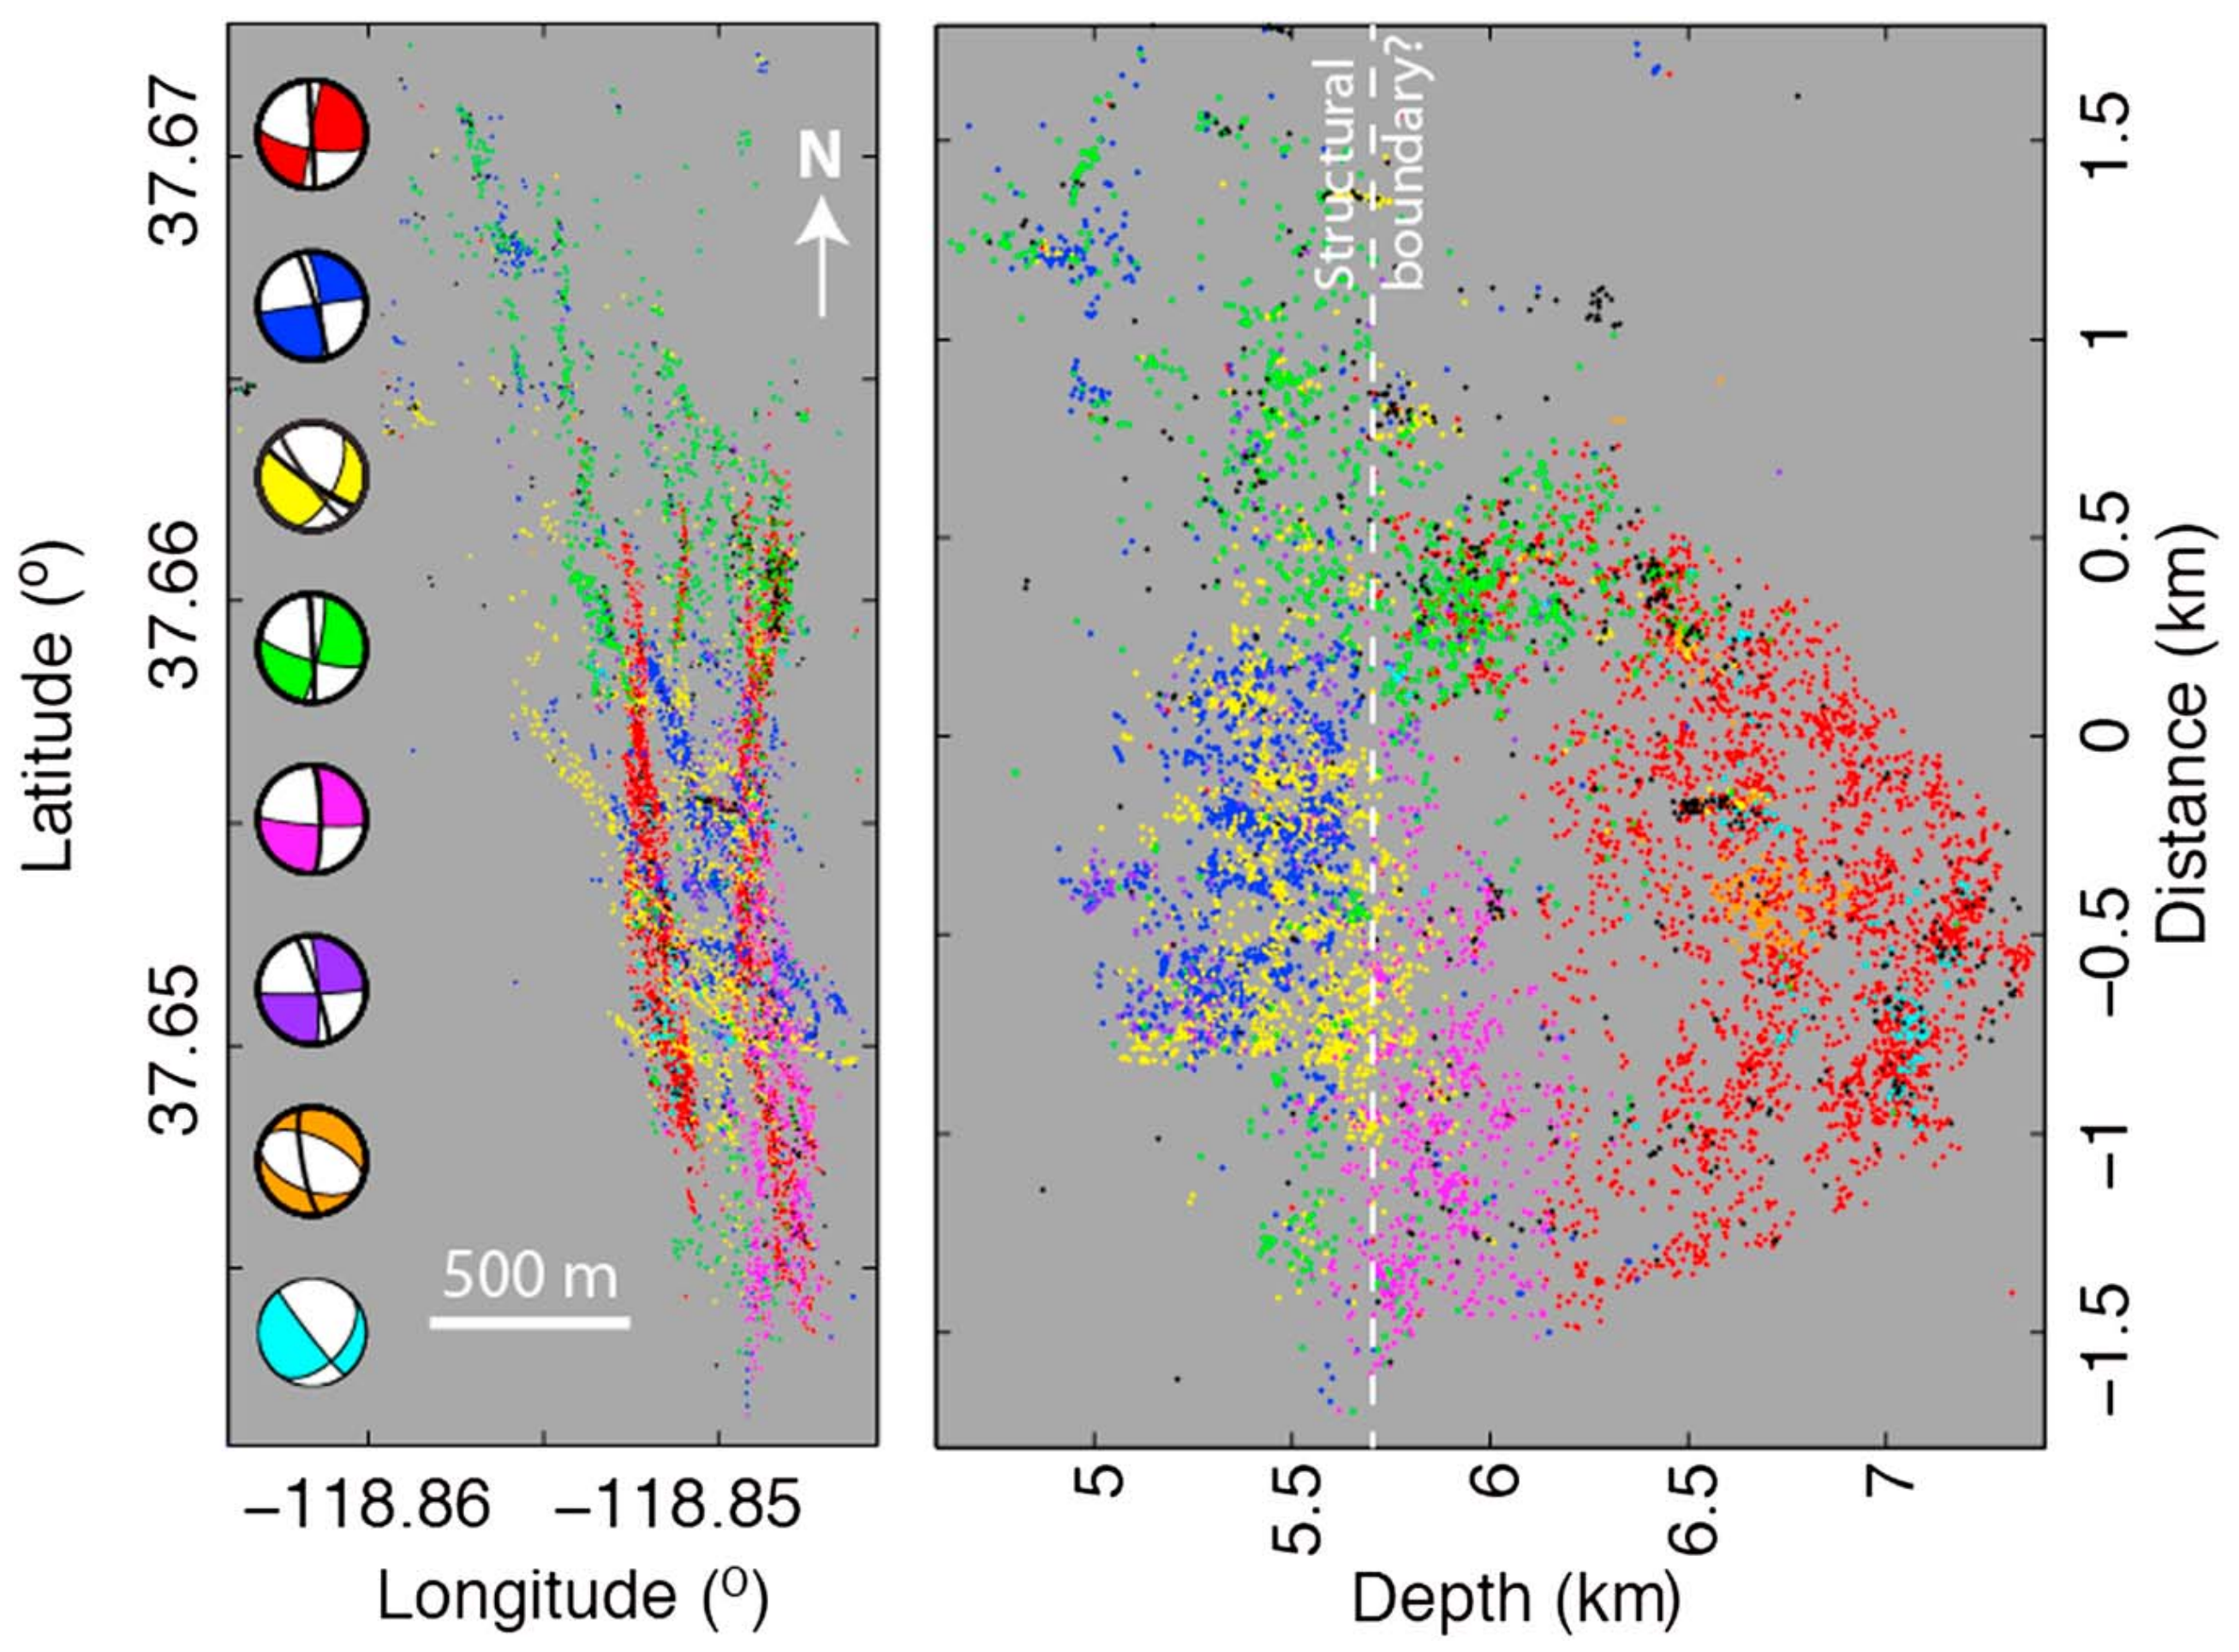
\includegraphics[width=1.00\columnwidth]{Chapter_6_Synthesis/figures/shelly_2016b_fig7/Shelly_2016b_fig7}
\caption[Polarity clustering output excerpted from \citet{Shelly_2016b}]{{
Figure excerpted from \citep{Shelly_2016b} showing the spatial distribution of event clusters determined using a waveform-correlation-based polarity clustering technique. The focal mechanisms depicted to the left of the figure show the `correlation composite' mechanism for each of the eight clusters. The locations of the events in each cluster, shown in map view and cross-section, are color-coded to match their corresponding focal mechanism.
{\label{shelly2016fig7}}%
}}
\end{center}
\end{figure}\selectlanguage{english}

We think this approach can be successfully applied to our Ngatamariki and Rotokawa catalogs, and may realistically increase the number of focal mechanism observations by an order of magnitude. Specifically, we think that the patterns revealed by these focal mechanisms can provide a detailed understanding of the location and orientation of specific flow pathways in the fields. That \citet{Shelly_2016b,Hotovec_Ellis_2018,shelly2018illuminating} were able to reveal complex faulting patterns at a scale of 100s of meters and in geologic settings similar to that of the \acrshort{TVZ} lends confidence to the potential for implementing this methodology at Rotokawa and Ngatamariki. In addition, the seismic network used in the aforementioned studies was more sparse than the network used here, which may also bode well for the application of this methodology to our dataset. To this end, we have already written the necessary functionality and have begun to apply these methods to both the Ngatamariki and Rotokawa catalogs.  

\subsection{Thermo-hydro-mechanical modeling}
As discussed in Chapter 5, knowledge of the stress state within a geothermal reservoir is key to understanding which fractures and faults are critically-stressed, susceptible to slip and therefore more likely to serve as fluid flow pathways. We have made a case for the use of earthquake focal mechanism inversion as a tool for monitoring reservoir stresses at Rotokawa and Ngatamariki, but have little stress data with which to verify our results. While \citet{davidson_2012} and \citet{McNamara_2015} have characterized certain aspects of the stress field at Rotokawa, the results are constrained only to certain wells in the aseismic production field and are therefore of limited use for constraining our focal mechanism inversions that are located in a separate reservoir compartment.

Geothermal operators heavily rely on numerical reservoir modeling for projecting field performance and developing production\slash{injection} strategies \citep{Grant_2011,DiPippo_2016}. At a minimum, these models simulate heat and multi-phase fluid flow in fractured and porous media, but variations of the most popular software packages (e.g. TOUGH, FEHM) also integrate equations for mass transfer, allowing for the simulation of the coupled thermo-hydro-mechanical system \citep{zyvoloski2007fehm,jung2017tough3}. It is therefore possible to simulate the state of stress in a reservoir during injection and production, while taking into consideration reservoir contraction due to cooling, which we and others have suggested dominates the induced stress change within a geothermal reservoir \citep{stephens1982hydraulic,Jeanne_2014,Mart_nez_Garz_n_2013,Mart_nez_Garz_n_2014,Jeanne_2015tensor,Jeanne_2015deformation}.

Simulating selected injection operations of interest at Rotokawa and Ngatamariki using these techniques would be valuable for assessing the mechanisms of stress change in the reservoir. Of particular interest are the northern injection wells (NM08, NM09) at Ngatamariki, due to the unexpected stress states observed from focal mechanism inversions in this part of the field. By simulating the stress variation due to cold water injection, we could assess if reservoir contraction is a realistic cause of stress change, or if the emplacement of the intrusive body is a more likely mechanisms of stress change. We have begun the process of modeling the \gls{stimulation} of NM08 using the finite element program \textit{FEHM} \citep{zyvoloski2007fehm}(Figure \ref{modeling}), and plan to extend these tests to include \gls{stimulation} and plant startup at NM09 as well. Currently, the model is being treated as a series of horizontal units with differing \gls{permeability}. However, we also plan to simulate discrete faults, constrained by the locations of seismicity, as dipping zones of increased \gls{permeability} extending across geologic units.

\begin{figure}[h!]
\begin{center}
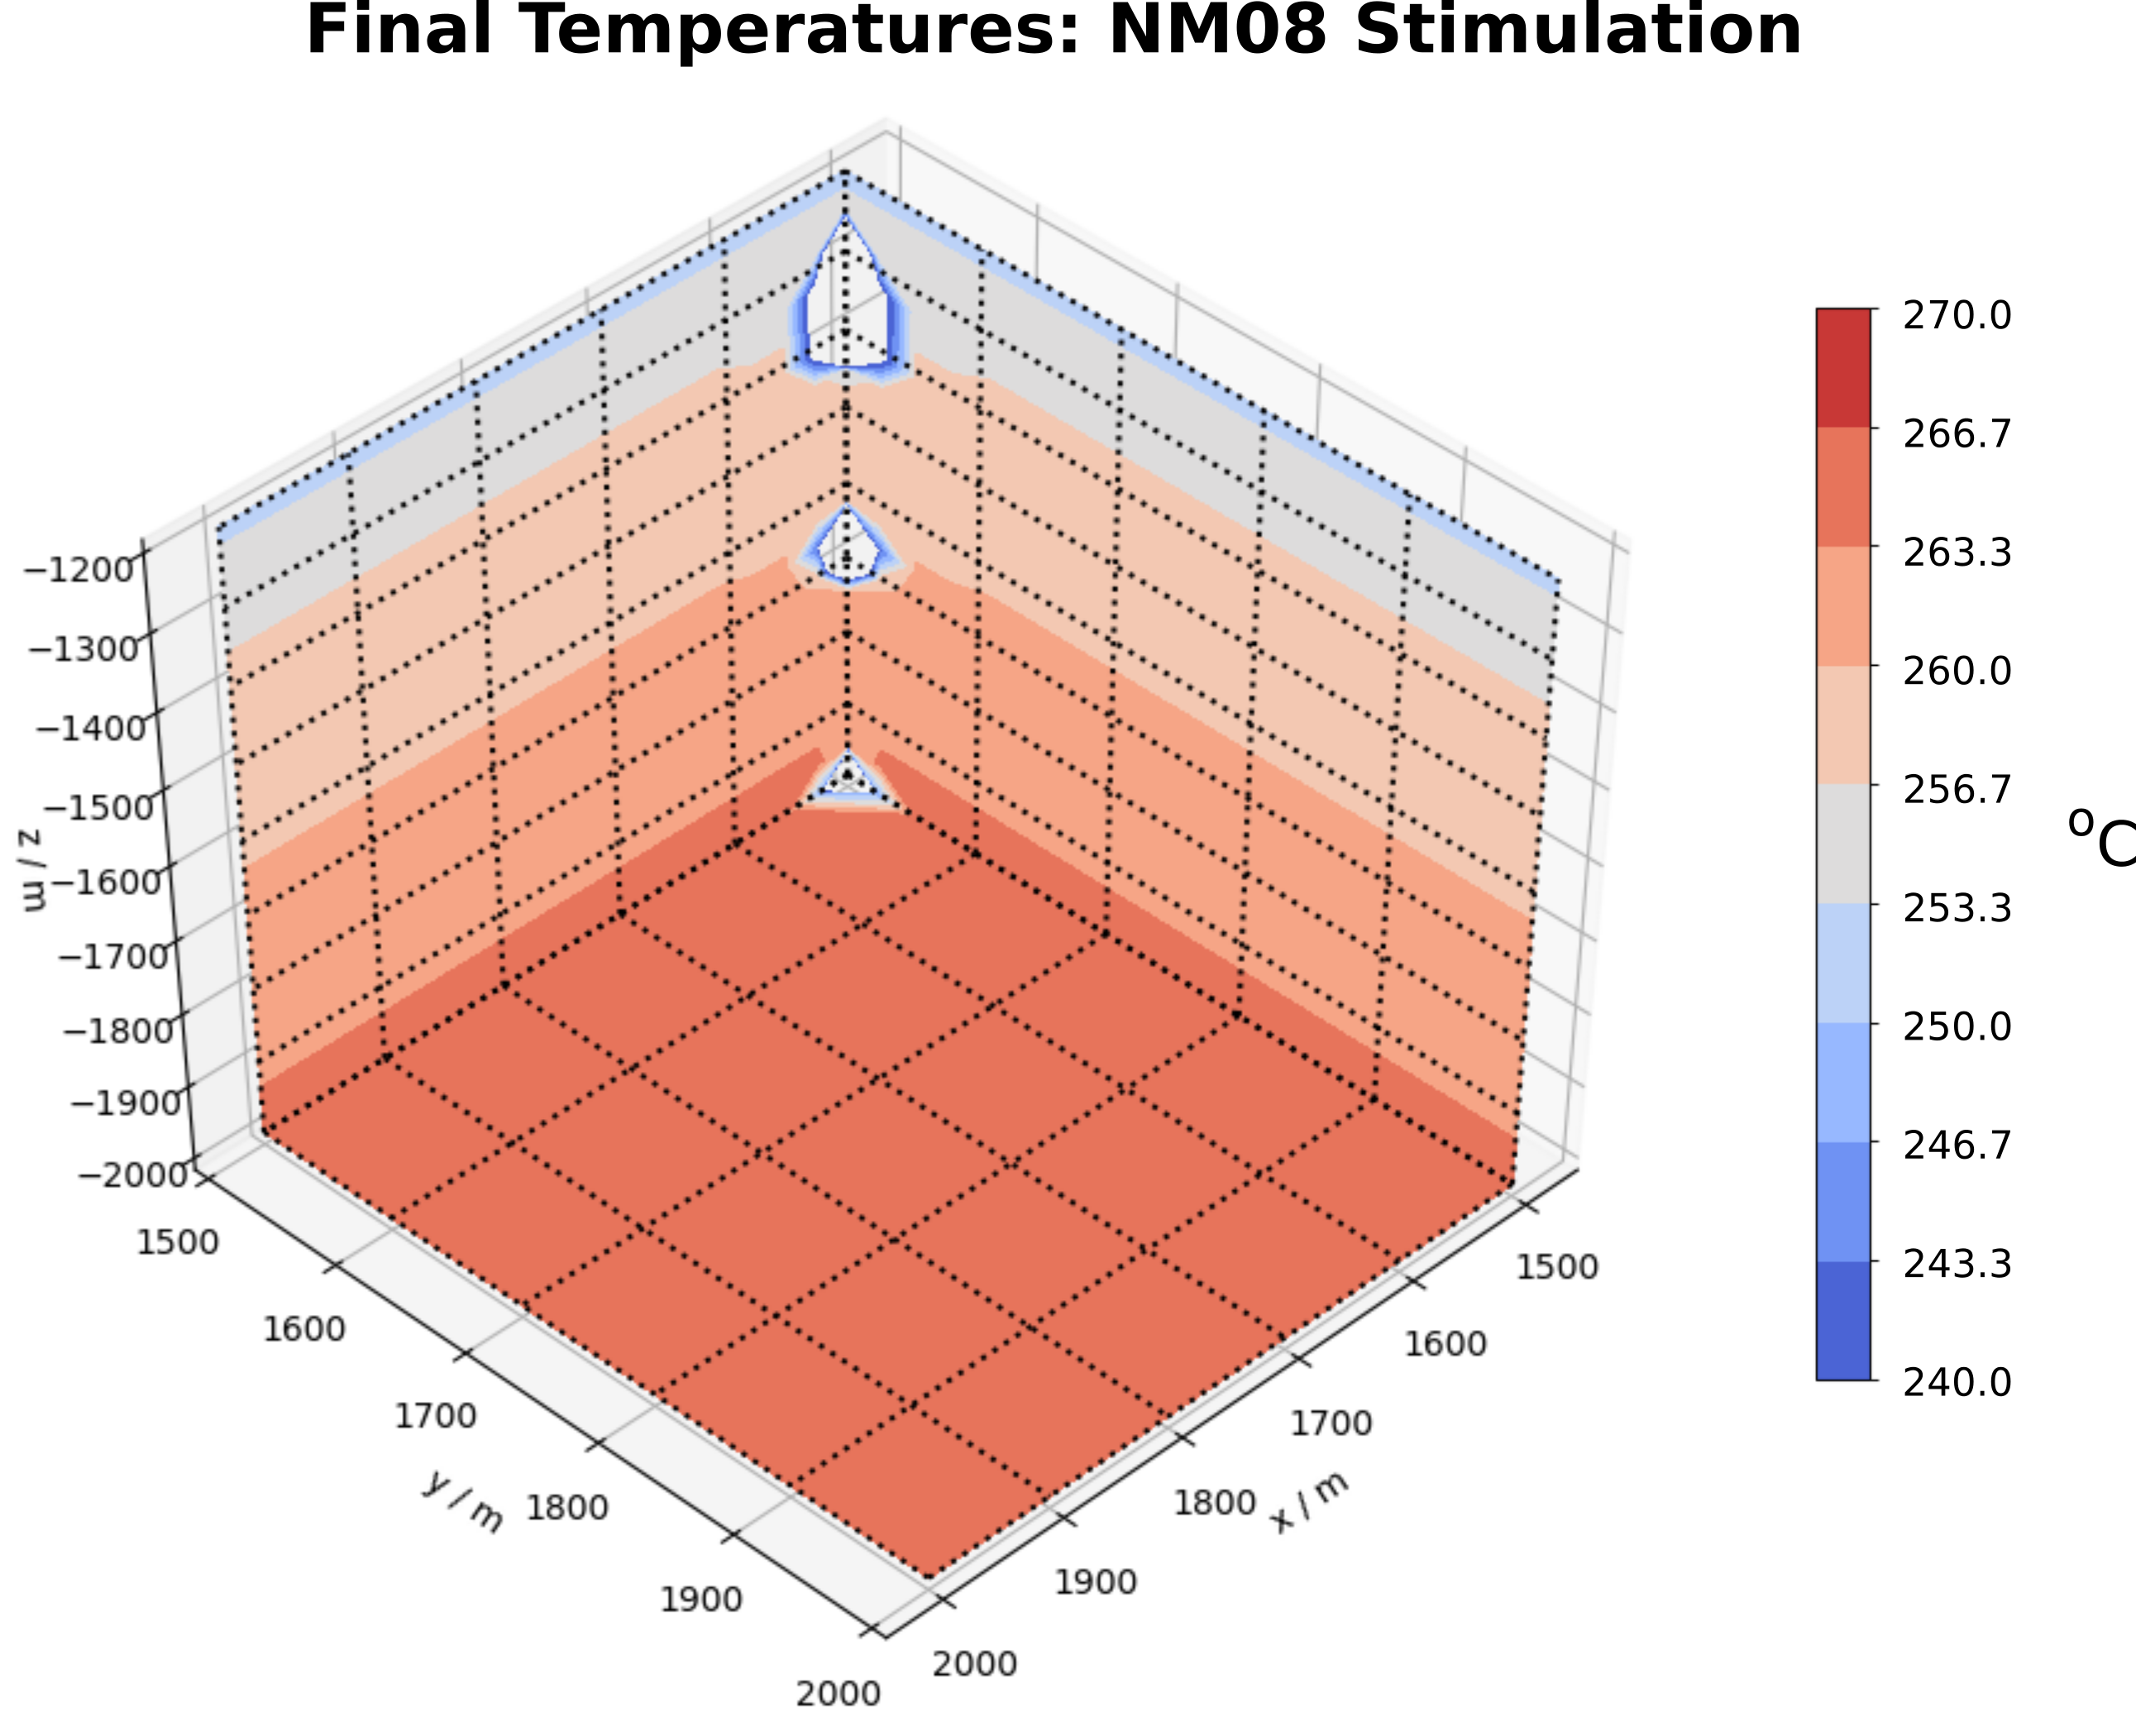
\includegraphics[width=1.00\columnwidth]{Chapter_6_Synthesis/figures/modeling_results/NM08_FEHM_output}
\caption[Example \textit{FEHM} temperature output]{{
Example temperature output from finite element modeling software \textit{FEHM} \citep{zyvoloski2007fehm} for northern Ngatamariki, following the \gls{stimulation} of NM08. The cooled zones correspond to the \glspl{feedzone} in the well as interpreted from \acrshort{PTS} runs. The model shown here contains four flat-lying geologic units representing surface deposits, a low \gls{permeability} clay cap, the Tahorakuri Formation and a tonalite intrusive body, with increasing depth, respectively. Lateral \gls{permeability} is anisotropic, and greater in the `y' direction than the `x' in order to simulate increased \gls{permeability} in subparallel to S$_{Hmax}$. We intend to extend this rather basic model to include faults (inferred from earthquake hypocenters) as high-permeability zones and additional wells, such as NM09. Pressure and temperature data from monitoring well NM02 may also be used to constrain the results of the simulation. Ideally, the modeled stresses will be compared to the stress inversion results for the kmeans clusters presented in Chapter 5.
{\label{modeling}}%
}}
\end{center}
\end{figure}\selectlanguage{english}

Modeling at Rotokawa is more complicated than at Ngatamariki, due mostly to decades of production prior to our study period, which has had an unknown effect on the stress state in the reservoir. However, we have better temporal stress resolution from focal mechanism inversion at Rotokawa than Ngatamariki. As a result, we may be able to compare the observed stress changes in the southeast compartment at Rotokawa with numerical modeling of wells RK20, 23 and 24. Specifically, we would look to answer the following questions regarding this section of the reservoir:
\begin{itemize}
    \item Are the observed stress ratio changes (interpreted to be related to injection at RK23) realistic and, if so, for what initial conditions can our stress inversions be matched (i.e. fracture spacing, initial stress state)?
    \item Does the \acrfull{IFF} act as a flow barrier between RK23 and RK20/24? Is it necessary to explain the observed variations in stress, or can those variations be modeled for the case where all three wells are hydraulically well-connected?
    \item Are the observed variations in $b$-value at Rotokawa reflected in the simulated pressure distributions? Specifically, are areas of high pore-fluid pressure similar to areas of high b-value as has been suggested elsewhere \citep{Bachmann_2012}? Do we have to invoke other variables (e.g. fracture density\slash{orientation}) to explain $b$-value change in the reservoir?
\end{itemize}

\section{Concluding statement}
This thesis expands upon an automatically-processed earthquake catalog for the Rotokawa and Ngatamariki geothermal field in New Zealand, doubling the number of events and decreasing the hypocentral uncertainties. We relate the properties of this precisely-located catalog to changes in injection operations at both fields, including the start-up of the Ngatamariki power plant and major injection migrations at Rotokawa. This is the first work of its kind at Ngatamariki, providing a baseline against which future seismicity can be measured. At Rotokawa we update the orientation of important flow-bounding faults and provide evidence for pressure-comparmentalization of the injection field. The work provided herein will serve to inform reservoir modeling at Rotokawa and Ngatamariki and further the understanding of the relationship between geothermal power production and seismicity more generally.